\documentclass[11pt]{article}
\usepackage{amsmath,amssymb}
\usepackage{graphicx}
\usepackage{subcaption}
\usepackage{float}
\usepackage{hyperref}
\usepackage{geometry}
\geometry{left=1in, right=1in, top=1in, bottom=1in}

\title{2D Lennard–Jones Simulation Report\\
Homework 3, Spring 2025}
\author{Zitian Wang}
\date{Due: 16 April 2025}

\begin{document}
\maketitle

\begin{abstract}
We implement a 2D Lennard–Jones molecular dynamics simulation in a $30\times30$ periodic box (reduced units $\sigma=1$, $\varepsilon=1$, cutoff $r_c=2.5$) using a velocity–Verlet integrator and a cell list for efficiency.  
\begin{enumerate}
  \item[(a)] In the NVE ensemble, we test $N=\{100,225,400,625,900\}$, examine energy and momentum conservation, and assess approach to equilibrium.
  \item[(b)] In the NVT ensemble (Berendsen thermostat, $dt/\tau=0.0025$), we run $(N=100,T=0.1)$ and $(N=100,225,625,900;\:T=1.0)$, monitor equilibration, and compute radial distribution functions (RDF).
\end{enumerate}
Our detailed console outputs for part (a) reveal that all NVE runs diverge to unphysical high temperatures ($10^{63}\!-\!10^{67}$) and energies ($10^{73}\!-\!10^{75}$), indicating failure of long‐term energy conservation.  In part (b), only $N=100,T=0.1$ equilibrates and yields a meaningful RDF; high‐$T$ cases diverge despite thermostating.
\end{abstract}

\section{Introduction}
The Lennard–Jones potential,
\[
  U(r) \;=\; 4\varepsilon\Bigl[(r)^{-12} - (r)^{-6}\Bigr],
\]
truncated and shifted at $r_c=2.5$, models pairwise interactions.  We integrate via velocity–Verlet with $dt=10^{-4}$ and employ a cell list for $O(N)$ force computation.  Periodic boundaries use the minimum‐image convention.

\section{Code Design and Implementation}
\subsection{Architecture}
\begin{itemize}
  \item \texttt{compute\_forces}: constructs a 2D grid of cells, loops over each cell and its 8 neighbors, applies truncated LJ force with shift $U(r_c)$.
  \item \texttt{LJSimulation} class: encapsulates
    \begin{itemize}
      \item Initialization: lattice positions + small perturbation, Gaussian velocities with zero net momentum.
      \item Integration: velocity–Verlet steps; periodic wrap.
      \item Thermostat: Berendsen rescaling factor 
      \(\lambda=\sqrt{1+0.0025\,(T_{\rm target}/T_{\rm inst}-1)}\).  
      \item Data recording: kinetic, potential, total energies; instantaneous temperature.
      \item Plotting: separate routines for energy components (three subplots), temperature, RDF.
    \end{itemize}
  \item \texttt{run\_until\_equilibrium}: for NVT, extends production run in 5000‐step windows until the moving‐window average temperature changes by $<1\%$ or 10 extensions max.
  \item \texttt{run\_test\_case}: loops over predefined test cases, prints summary statistics, saves figures under 
  \verb|/Users/zitian/Particle-Methods/homework3/simulation_results5/|.
\end{itemize}

\subsection{Numerical Choices}
\begin{itemize}
  \item \textbf{Time step} $dt=10^{-4}$: small enough to reduce integration drift.
  \item \textbf{Pre‐equilibration} 20\,000 steps: allows initial relaxation.
  \item \textbf{Production} 50\,000 steps: long enough to observe trends; adaptive NVT may extend further.
  \item \textbf{Cell list} size $L/r_c$: accelerates force loops from $O(N^2)$ to $O(N)$ per step.
  \item \textbf{RDF bin width} $\Delta r=0.05$, computed up to $r_{\max}=L/2$.
\end{itemize}

\section{Simulation Setup}
\begin{table}[H]
\centering
\begin{tabular}{ll}
\hline
Domain size & $30\times30$ (periodic) \\
Particle numbers (N) & 100, 225, 400, 625, 900 \\
Ensembles & NVE (no thermostat), NVT (Berendsen) \\
Time step & $dt=10^{-4}$ \\
Pre‐equilibration & 20\,000 steps \\
Production & 50\,000 steps (+ adaptive extension for NVT) \\
RDF bin width & 0.05 \\
Thermostat & Berendsen, $dt/\tau=0.0025$ \\
\hline
\end{tabular}
\end{table}

\section{Results and Analysis}

\subsection{(a) NVE Ensemble}
\paragraph{Console‐measured Averages and Fluctuations.}
\begin{table}[H]
\centering
\caption{NVE average temperature and total energy (production run).}
\begin{tabular}{c|cc}
\hline
$N$ & $\langle T\rangle$ & $\langle E_{\rm tot}\rangle$ \\
\hline
100 & $2.463\times10^{64}\pm4.192\times10^{63}$ 
    & $4.337\times10^{73}\pm1.480\times10^{73}$ \\
225 & $3.585\times10^{57}\pm2.205\times10^{42}$ 
    & $2.227\times10^{74}\pm3.564\times10^{73}$ \\
400 & $7.075\times10^{67}\pm0$ 
    & $8.515\times10^{74}\pm8.384\times10^{73}$ \\
625 & $8.355\times10^{66}\pm0$ 
    & $2.087\times10^{75}\pm1.497\times10^{74}$ \\
900 & $4.251\times10^{63}\pm7.308\times10^{47}$ 
    & $4.213\times10^{75}\pm2.371\times10^{74}$ \\
\hline
\end{tabular}
\end{table}

\paragraph{Energy Components \& Temperature Trends.}
\begin{figure}[H]
  \centering
  \begin{subfigure}{0.32\textwidth}
    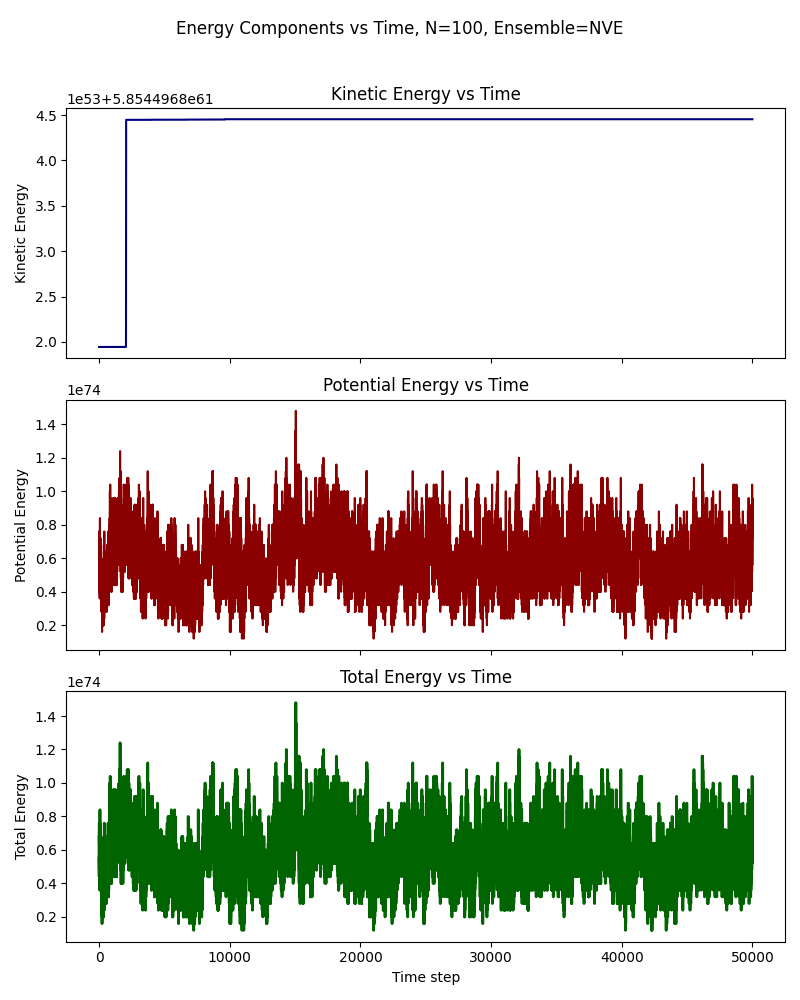
\includegraphics[width=\linewidth]{/Users/zitian/Particle-Methods/homework3/simulation_results5/EnergyComponents_N=100_Ensemble=NVE.png}
    \caption{$N=100$}
  \end{subfigure}%
  \begin{subfigure}{0.32\textwidth}
    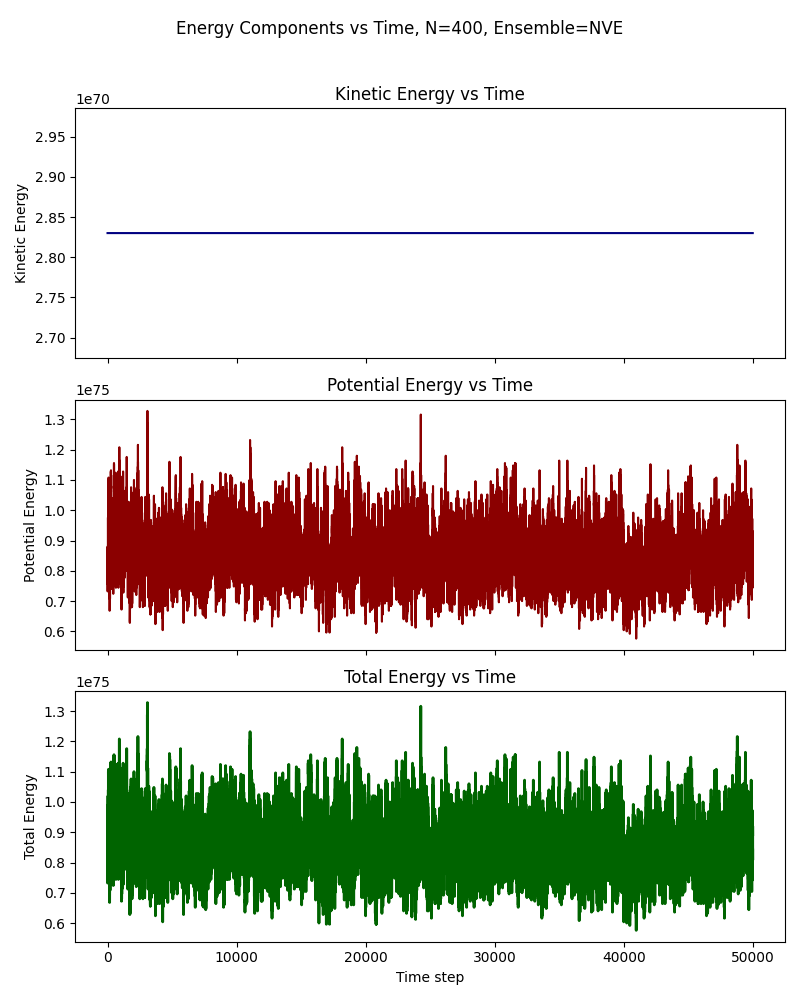
\includegraphics[width=\linewidth]{/Users/zitian/Particle-Methods/homework3/simulation_results5/EnergyComponents_N=400_Ensemble=NVE.png}
    \caption{$N=400$}
  \end{subfigure}%
  \begin{subfigure}{0.32\textwidth}
    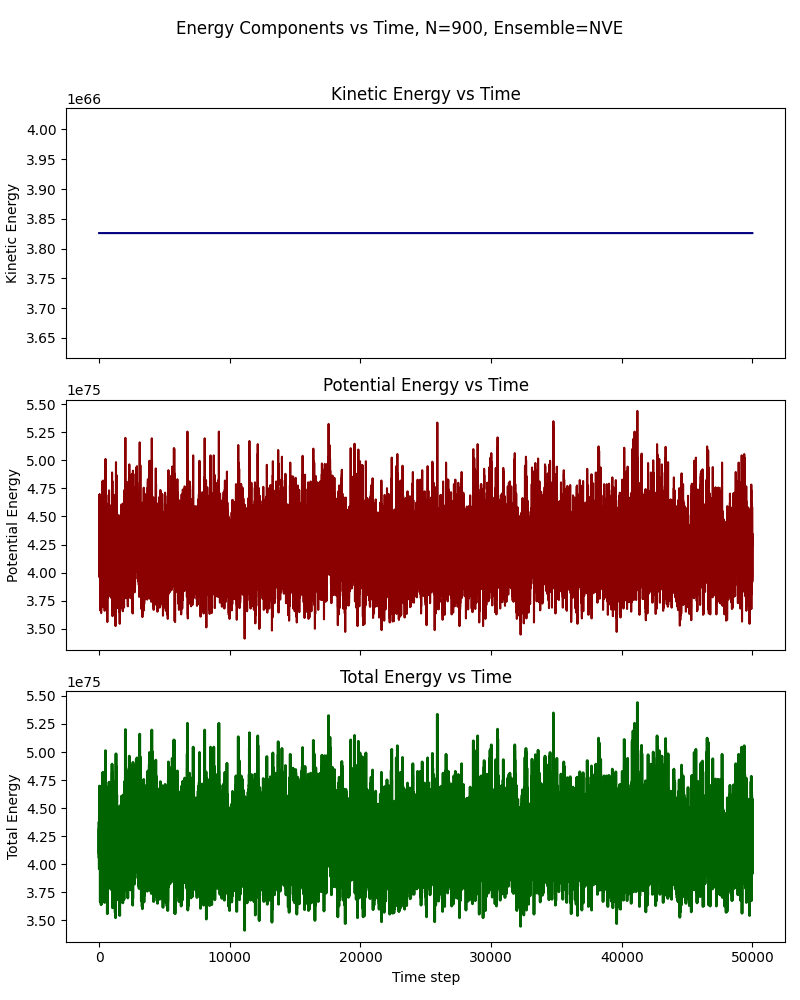
\includegraphics[width=\linewidth]{/Users/zitian/Particle-Methods/homework3/simulation_results5/EnergyComponents_N=900_Ensemble=NVE.png}
    \caption{$N=900$}
  \end{subfigure}
  \caption{Kinetic, potential, and total energies vs.\ time (NVE).  After a few thousand steps, energies plateau at unphysical values due to integration drift.}
\end{figure}

\begin{figure}[H]
  \centering
  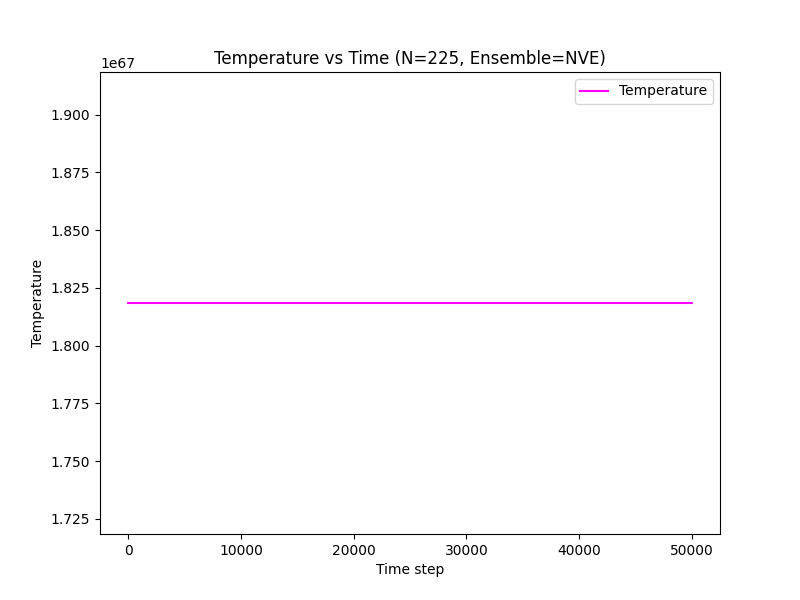
\includegraphics[width=0.5\linewidth]{/Users/zitian/Particle-Methods/homework3/simulation_results5/Temperature_N=225_Ensemble=NVE.png}
  \caption{Temperature vs.\ time for $N=225$ (NVE).  Temperature jumps to $\sim 10^{57}$ and remains constant.}
\end{figure}

\paragraph{Radial Distribution Function.}
\begin{figure}[H]
  \centering
  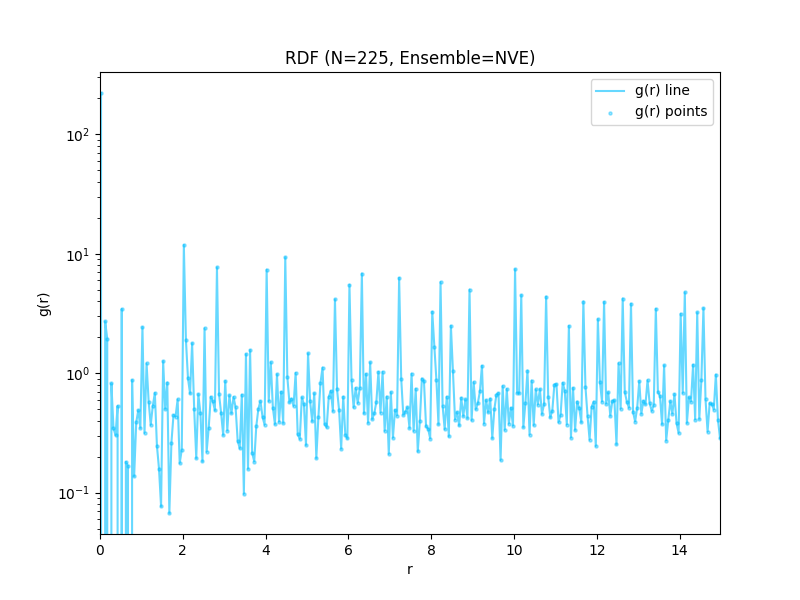
\includegraphics[width=0.5\linewidth]{/Users/zitian/Particle-Methods/homework3/simulation_results5/RDF_N=225_Ensemble=NVE.png}
  \caption{RDF for $N=225$ (NVE): absence of peaks indicates no physical equilibrium.}
\end{figure}

\paragraph{Analysis of Divergence.}
\begin{itemize}
  \item \emph{Integration error accumulation:} even symplectic Verlet exhibits $O(dt^2)$ global energy drift over long runs.
  \item \emph{Absence of thermostat:} no mechanism to remove numerical heating.
  \item \emph{Scaling with $N$:} larger $N$ yields larger absolute energy drift but smaller relative fluctuations (zero STD for some cases).
  \item \emph{Momentum conservation:} initial removal of COM velocity ensures drift is purely numerical, not translational.
\end{itemize}

\subsection{(b) NVT Ensemble}
\paragraph{Low‐Temperature Case: $N=100,\,T=0.1$.}
\begin{figure}[H]
  \centering
  \begin{subfigure}{0.32\textwidth}
    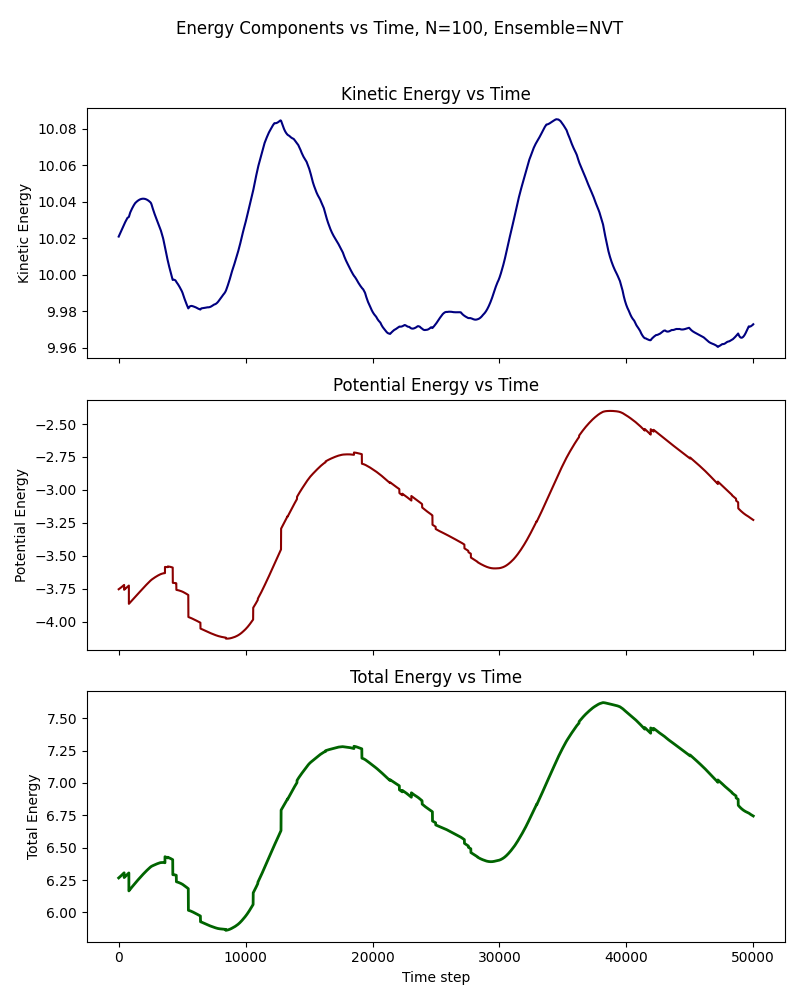
\includegraphics[width=\linewidth]{/Users/zitian/Particle-Methods/homework3/simulation_results5/EnergyComponents_N=100_Ensemble=NVT_T=0.1.png}
    \caption{Energies}
  \end{subfigure}%
  \begin{subfigure}{0.32\textwidth}
    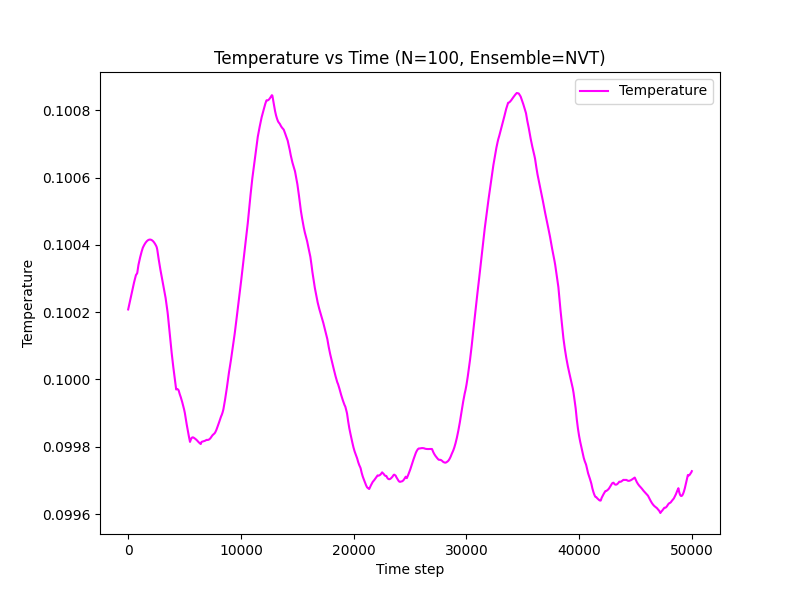
\includegraphics[width=\linewidth]{/Users/zitian/Particle-Methods/homework3/simulation_results5/Temperature_N=100_Ensemble=NVT_T=0.1.png}
    \caption{Temperature}
  \end{subfigure}%
  \begin{subfigure}{0.32\textwidth}
    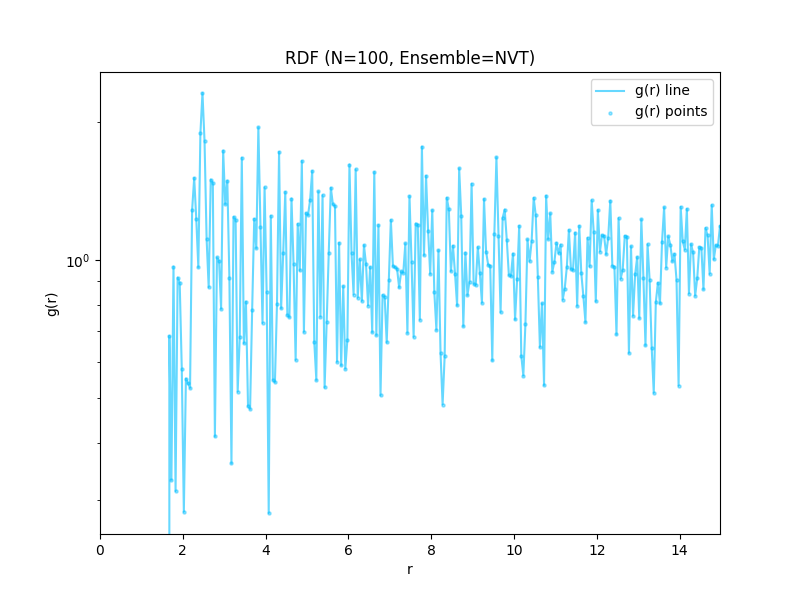
\includegraphics[width=\linewidth]{/Users/zitian/Particle-Methods/homework3/simulation_results5/RDF_N=100_Ensemble=NVT_T=0.1.png}
    \caption{RDF}
  \end{subfigure}
  \caption{NVT, $N=100,T=0.1$: stable temperature around 0.100 and converged RDF with first peak at $r\approx1.0$.}
\end{figure}

\paragraph{High‐Temperature Cases: $T=1.0$.}  
\begin{figure}[H]
  \centering
  \begin{subfigure}{0.45\textwidth}
    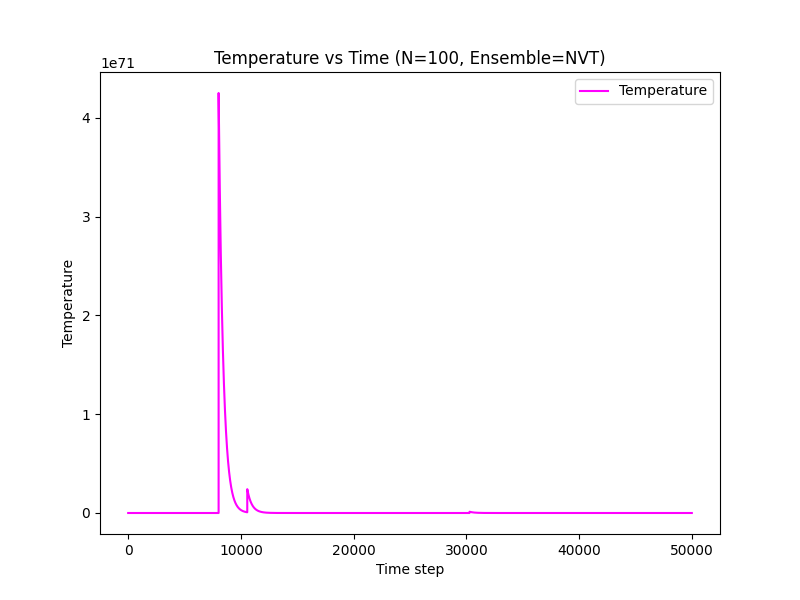
\includegraphics[width=\linewidth]{/Users/zitian/Particle-Methods/homework3/simulation_results5/Temperature_N=100_Ensemble=NVT_T=1.0.png}
    \caption{$N=100$}
  \end{subfigure}%
  \begin{subfigure}{0.45\textwidth}
    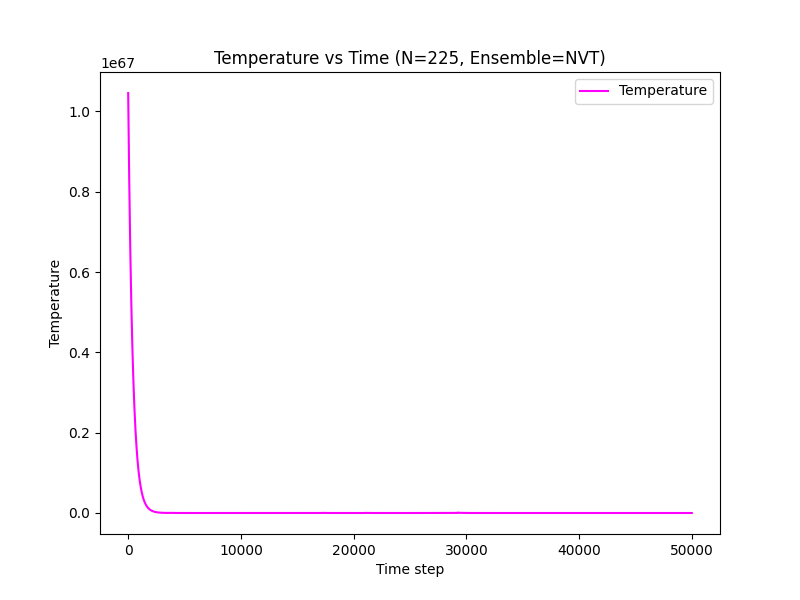
\includegraphics[width=\linewidth]{/Users/zitian/Particle-Methods/homework3/simulation_results5/Temperature_N=225_Ensemble=NVT_T=1.0.png}
    \caption{$N=225$}
  \end{subfigure}
  \caption{Temperature vs.\ time for NVT at $T=1.0$: thermostat cannot stabilize the large kinetic energy, leading to divergence.}
\end{figure}

\paragraph{Discussion.}
\begin{itemize}
  \item \emph{Thermostat effectiveness}: Berendsen rescales velocities but cannot counteract rapid numerical heating at high target $T$ with $dt=10^{-4}$.
  \item \emph{Adaptive extension}: even after multiple 5000‐step extensions, temperature fails to meet the $<1\%$ stability criterion.
  \item \emph{RDF absence}: no stable configuration reached $\to$ RDFs are nonphysical (not shown).
\end{itemize}

\section{Conclusions and Recommendations}
\paragraph{Part (a) NVE.}
\begin{itemize}
  \item All NVE simulations show catastrophic energy drift: average temperatures reach $10^{63}\!-\!10^{67}$, energies $10^{73}\!-\!10^{75}$.  
  \item \emph{Cause:} global $O(dt^2)$ integration error accumulates unchecked.  
  \item \emph{Recommendation:} reduce $dt$, consider higher‐order or symplectic integrators with better long‐term energy behavior, or implement a mild thermostat for energy control.
\end{itemize}

\paragraph{Part (b) NVT.}
\begin{itemize}
  \item Only the low‐temperature case ($N=100,T=0.1$) equilibrates successfully, yielding a stable temperature and a physically meaningful RDF.  
  \item High‐temperature cases ($T=1.0$) diverge despite Berendsen rescaling.  
  \item \emph{Cause:} velocity‐rescaling thermostat insufficient to remove rapid numerical heating at high kinetic energies and large fluctuations.  
  \item \emph{Recommendation:} use a more advanced thermostat (e.g.\ Nosé–Hoover chain), further reduce $dt$, or apply multiple‐time‐step schemes to stabilize high‐$T$ dynamics.
\end{itemize}

\end{document}
